\documentclass[dvipdfmx]{jsarticle}
\usepackage[T1]{fontenc}
\usepackage[dvipdfmx]{hyperref}
\usepackage{lmodern}
\usepackage{latexsym}
\usepackage{amsfonts}
\usepackage{amssymb}
\usepackage{mathtools}
\usepackage{amsthm}
\usepackage{multirow}
\usepackage{graphicx}
\usepackage{wrapfig}
\usepackage{here}
\usepackage{float}
\usepackage{ascmac}
\usepackage{url}

\title{統計学1 中間課題 答案(再提出)}
\author{文理学部 情報科学科\\5419045 高林 秀}
\date{\today}

\begin{document}

\maketitle

\begin{abstract}
    本稿は、後期総合教育科目である統計学1の中間課題として与えられた、健康診断データの分析に関するレポートである。\par 
    平均や、標準偏差といった各種指標数値の計算にはPythonのライブラリであるPandasを用いて計算を行った。また、グラフの描画にはmatplotlibを使用した。\par 
    はじめに、各数値データ(年齢、身長、体重、最大血圧、最小血圧)に関して、それぞれ平均や標準偏差、度数分布表、ヒストグラムを作成し、元データ全体がどのような分布になっているかについて考察した。 
    その後、各数値(量的)データと質的データ(以降は「血圧判定」「心電図判定」を指す)の関連性を調べるため、相関比を算出し、結果から導かれることを考察した。
\end{abstract}

\tableofcontents
\newpage
\section{各データの概要}

    この章では、健康診断データの全体像を把握するため、平均や標準偏差、ヒストグラム、クロス集計表を用いて、各データの分布を可視化した。\par
    また、可視化したデータを分析し、その結果から導かれることを考察した。
    \subsection{各数値データの概要}
    まず、以下の表に性別を区別しない場合、男性のみのデータ、女性のみのデータでそれぞれの平均や標準偏差、最大値、最小値を算出した。
    \begin{table}[H]
        \caption{性別の区別がない場合の平均・標準偏差・最大,最小値}
        \centering
        \begin{tabular}{lccccc}
            & \multicolumn{1}{r}{年齢} & \multicolumn{1}{r}{身長(cm)} & \multicolumn{1}{r}{体重(kg)} & \multicolumn{1}{r}{最大血圧(mmHg)} & \multicolumn{1}{r}{最小血圧(mmHg)} \\
        平均   & 41.3                   & 162.5                  & 60.3                   & 124.9                    & 89.4                     \\
        標準偏差 & 12.1                   & 10.2                   & 9.4                    & 9.2                      & 15.2                     \\
        最大値  & 67.0                   & 185.0                  & 75.0                   & 144.0                    & 129.0                    \\
        最小値  & 23.0                   & 141.0                  & 43.0                   & 105.0                    & 65.0                     \\
        \hline
        総数 & 50 &  &  &  &  

    \end{tabular}
    \end{table}
    \begin{table}[H]
        \caption{男性のみのデータの平均・標準偏差・最大,最小値}
        \centering
        \begin{tabular}{lccccc}

            & \multicolumn{1}{r}{年齢} & \multicolumn{1}{r}{身長(cm)} & \multicolumn{1}{r}{体重(kg)} & \multicolumn{1}{r}{最大血圧(mmHg)} & \multicolumn{1}{r}{最小血圧(mmHg)} \\
        平均   & 40.0                   & 170.0                  & 66.0                   & 126.6                    & 87.0                     \\
        標準偏差 & 11.2                   & 6.2                    & 5.6                    & 9.3                      & 13.9                     \\
        最大値  & 67.0                   & 185.0                  & 75.0                   & 75.0                     & 125.0                    \\
        最小値  & 23.0                   & 159.0                  & 53.0                   & 115.0                    & 65.0                     \\
        \hline
        総数 & 24 &  &  &  & 
    \end{tabular}
    \end{table}
    \begin{table}[H]
        \caption{女性のみのデータの平均・標準偏差・最大,最小値}
        \centering
        \begin{tabular}{llllll}
            & \multicolumn{1}{r}{年齢} & \multicolumn{1}{r}{身長(cm)} & \multicolumn{1}{r}{体重(kg)} & \multicolumn{1}{r}{最大血圧(mmHg)} & \multicolumn{1}{r}{最小血圧(mmHg)} \\
        平均   & 41.7                   & 155.7                  & 55.0                   & 123.3                    & 91.6                     \\
        標準偏差 & 13.0                   & 8.2                    & 9.2                    & 8.9                      & 16.3                     \\
        最大値  & 65.0                   & 172.0                  & 75.0                   & 143.0                    & 129.0                    \\
        最小値  & 23.0                   & 141.0                  & 43.0                   & 105.0                    & 65.0                    \\
        \hline
        総数 & 26 &  &  &  &
        \end{tabular}
    \end{table}
    続いて、上記の3パターンで、各数値データのヒストグラムを示す。度数分布表は画像のサイズが大きい為、省略する。
    \begin{figure}[H]
        \centering
        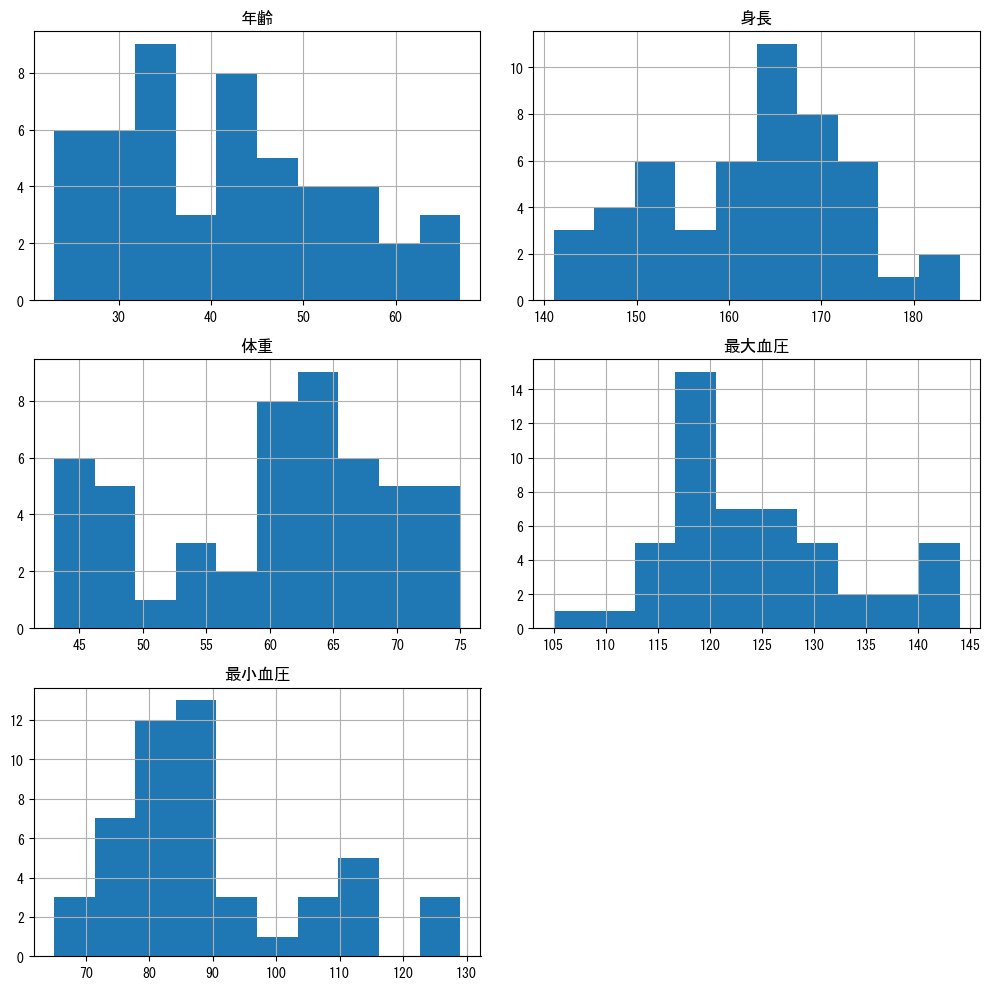
\includegraphics[scale=0.6]{./images/allgender/hist.png}
        \caption{全性別でのヒストグラム}
    \end{figure}
    \begin{figure}[H]
        \centering
        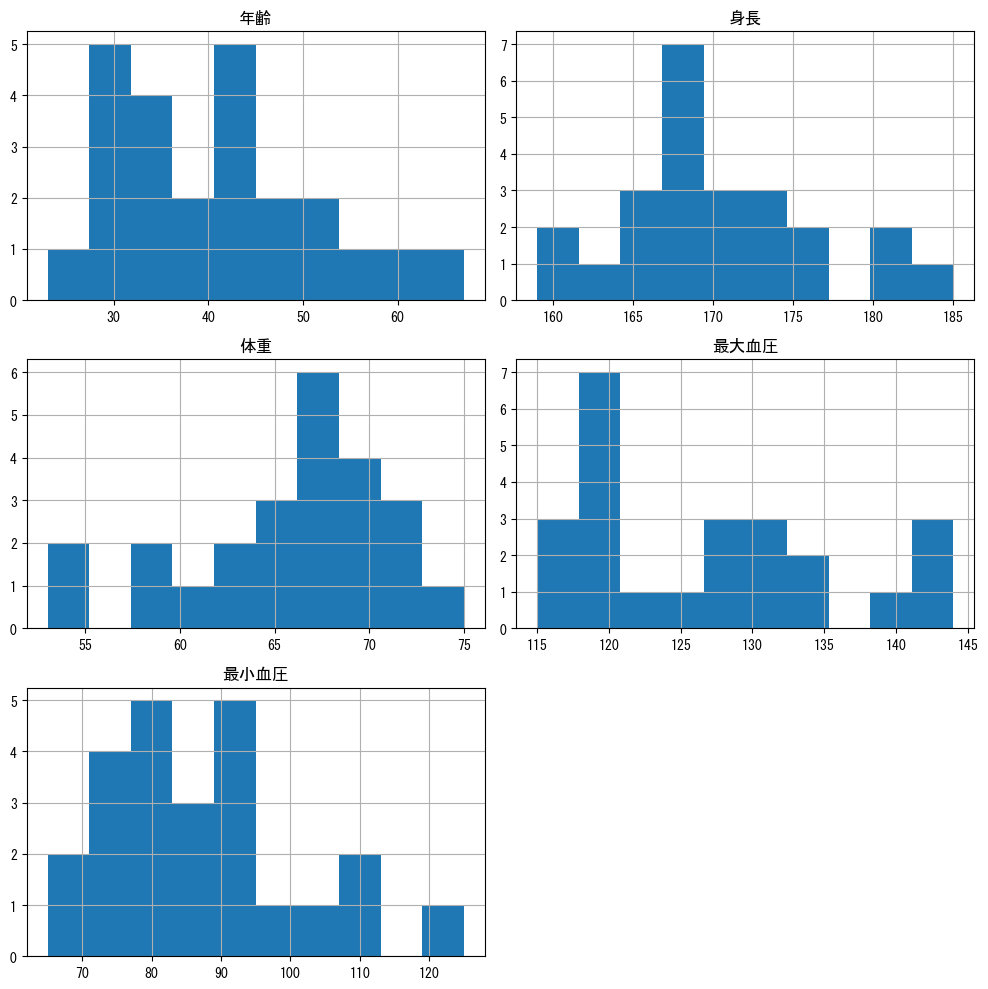
\includegraphics[scale=0.6]{./images/male/hist.png}
        \caption{男性データのヒストグラム}
    \end{figure}
    \begin{figure}[H]
        \centering
        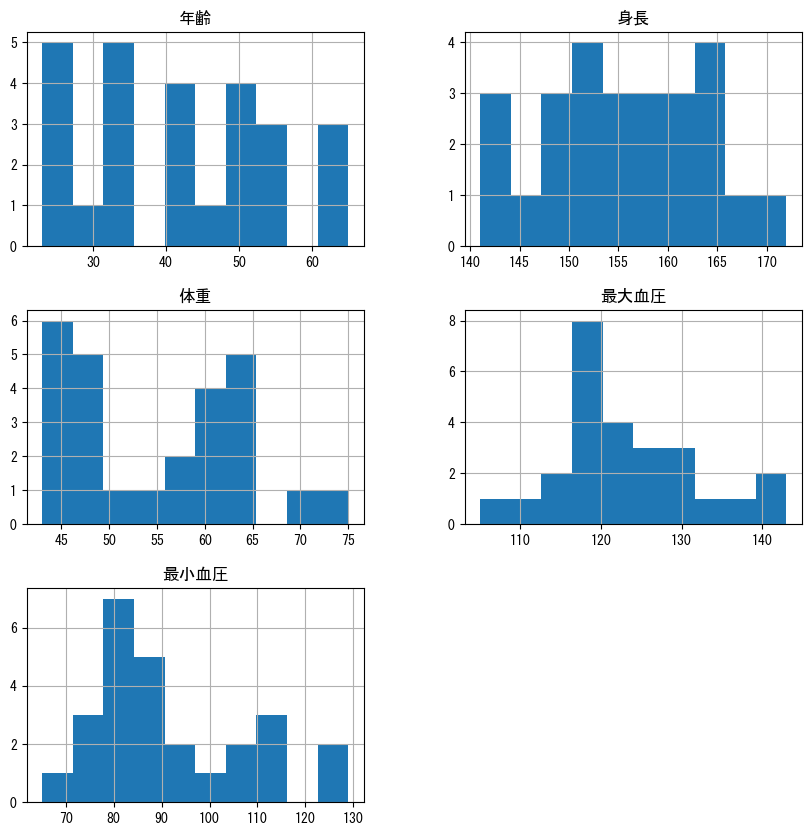
\includegraphics[scale=0.6]{./images/female/hist.png}
        \caption{女性データのヒストグラム}
    \end{figure}
\newpage
    \subsubsection{年齢ごとの身長・体重・最大,最小血圧値の対応}
    続いて、年齢ごとの身長・体重・最大,最小血圧値の推移を折れ線グラフで可視化した。その結果を以下に示す。
    \begin{figure}[H]
        \centering
        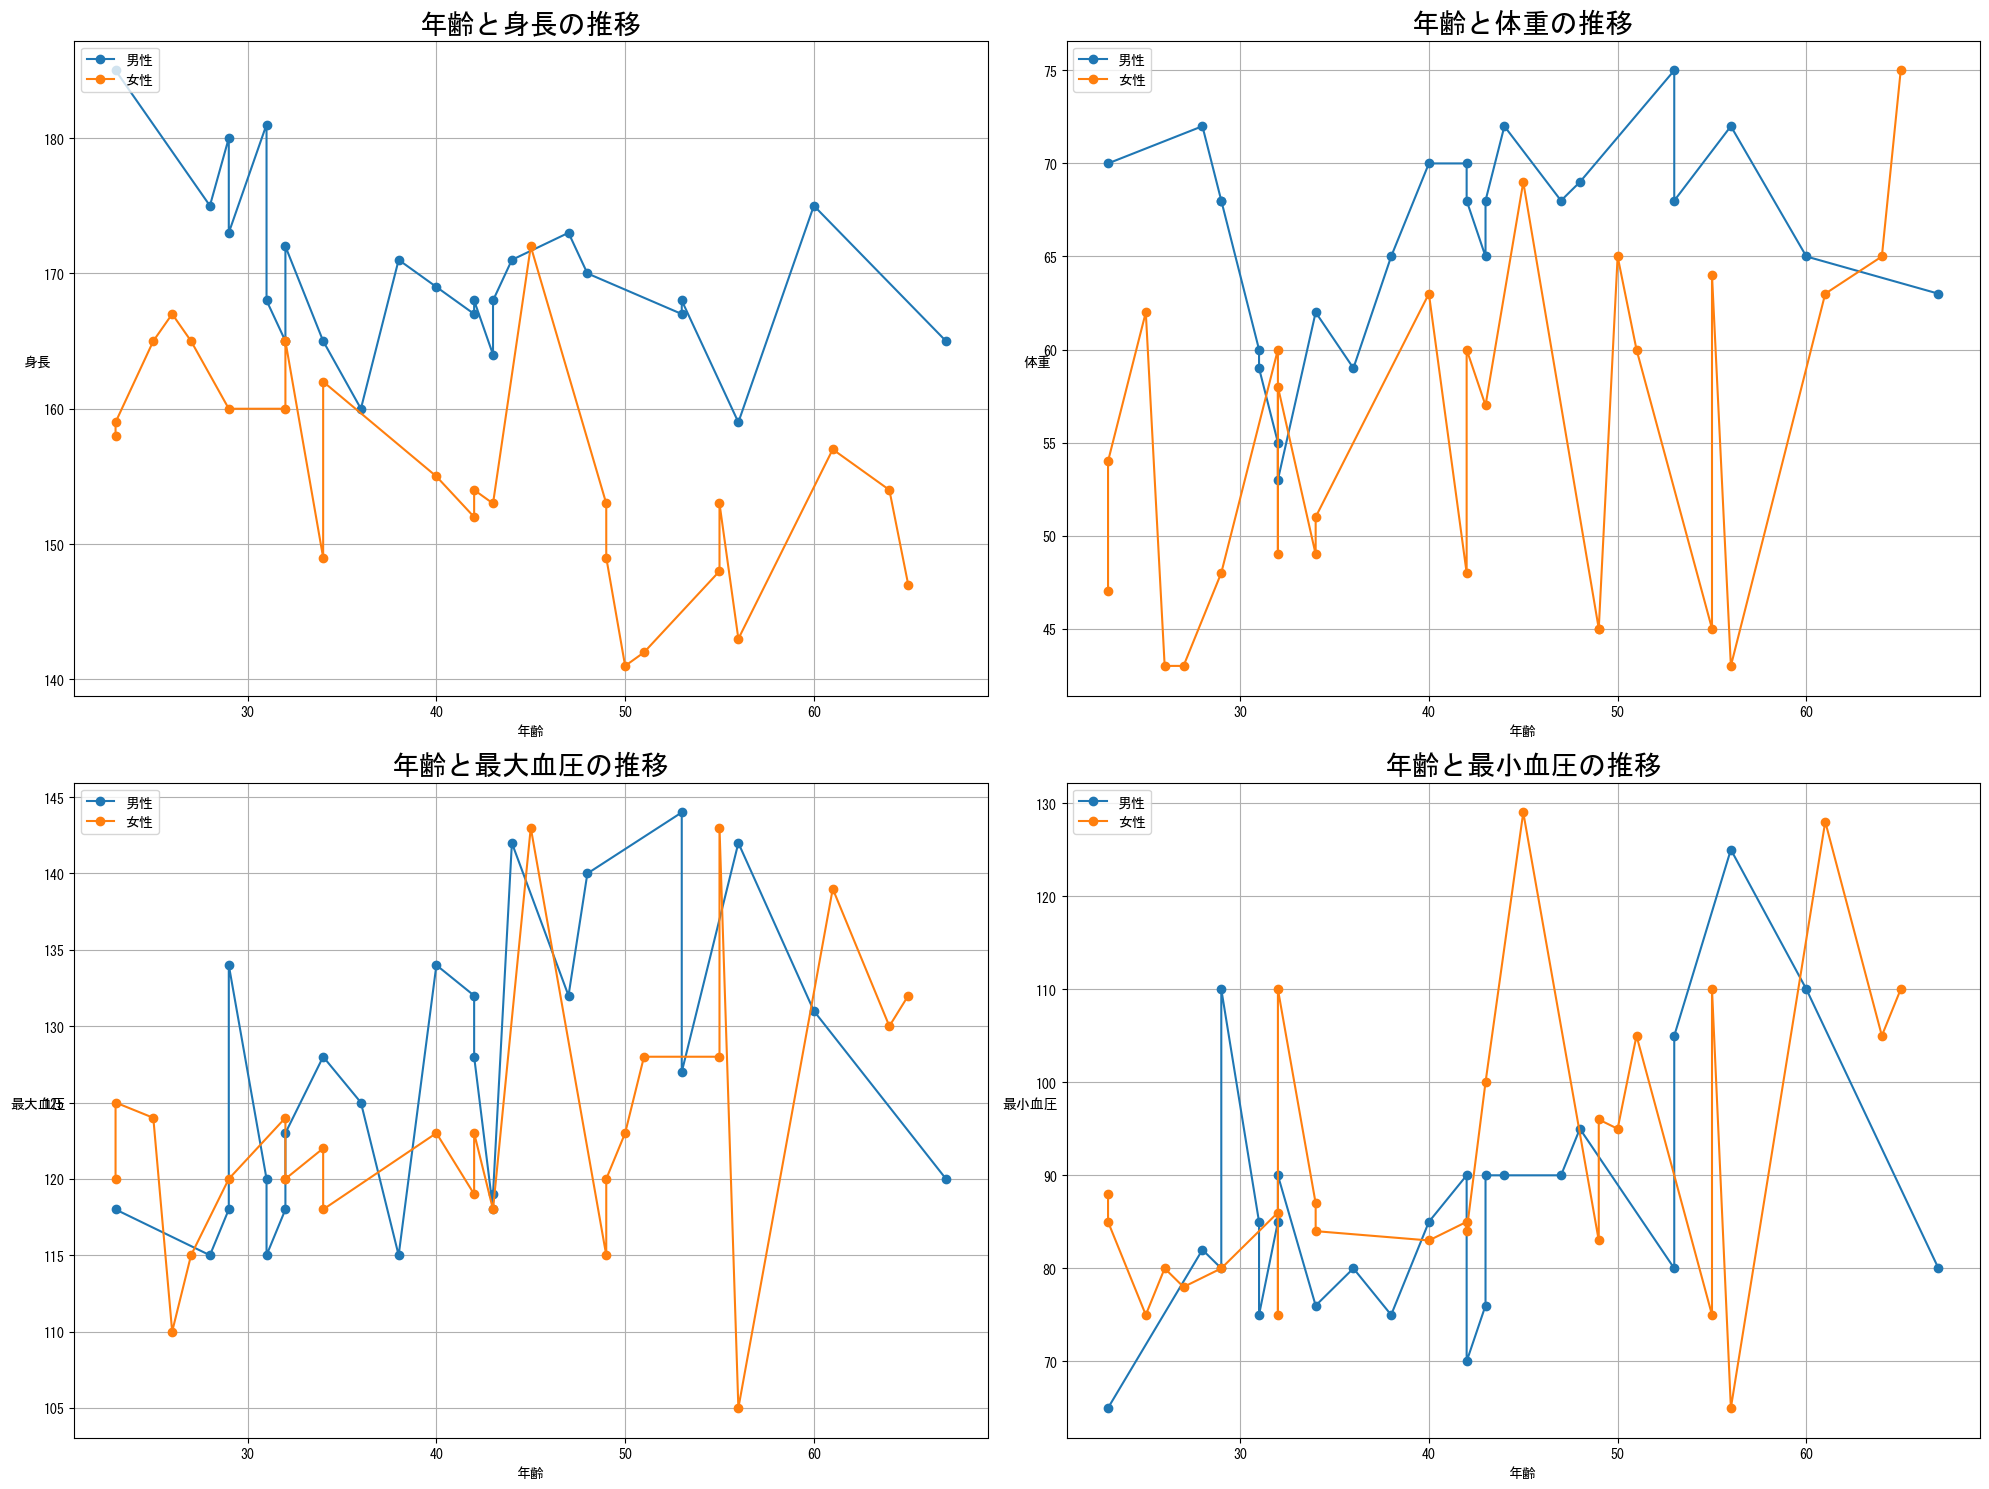
\includegraphics[scale=0.32]{images/allgender/age_tarnsition.png}
        \caption{年齢ごとの身長・体重・最大,最小血圧値の対応}
    \end{figure}
    このグラフから、本課題で使用したデータにおいて、年齢とそれ以外の各数値データの関係性に関して以下のことが言える。以下の考察はあくまで本データに対してのみであり、一般的なこととは限らない。
    \paragraph{年齢と身長}
    男性の場合は、年齢が上昇するにつれて全体として身長が下がっている傾向があるのが分かる。30代以下の人の身長の値は大体180cm~170cmの間であるのに対し、50代以上になると160cm~170cmの間の人が多く、年齢が大きくなるにつれて身長が下がっていく傾向がある。
    また、一般的に「高身長」といわれる身長175cm以上の人は、今回のデータでは30代以下がほとんどで、それ以上になると170cm程度の人が多いことが分かる。\par
    女性の場合も同様で、年齢が上昇するにつれて全体として身長が下がっている傾向があるのが分かる。30代以下の人の身長の値は大体160cm~170cmの間であるのに対し、50代以上になると140cm~150cmの間の人が多く、年齢が大きくなるにつれて身長が下がっていく傾向がある。\par
    また、性別によって、同じ年代でも身長大きさにはかなり開きがあることがこのグラフから明らかになった。特に、30代以下の人と、50代以上の人のデータにおいて、男性の身長は女性の身長よりも大きい傾向があることが分かる。
    \paragraph{年齢と体重}
    男性の場合は、女性に比べ比較的年代ごとに体重は同じような値をとっていることがグラフから分かる。例えば、40代~50代の人は大体体重65kg~70kgの間にある人が多い。反対に、女性の場合は同じ年代の人同士でも、体重の値に明かな開きがあることが分かる。
    例えば40代~50代の人は、体重の値が、下は45kg程度で上は70kg弱といったように、体重の値にかなりの開きがある。\par 
    また、男性の場合は、50代後半の人から、体重の値が下がっていく傾向にあるのに対し、女性の場合は反対に増えているのが分かる。この原因として以下の文章の現象が関係していそうなので引用する。
    \begin{quote}
        閉経を迎えると女性ホルモンよりも男性ホルモン優位となることが関係し、中性脂肪をため込みやすい体質に変化。また、基礎代謝量の減少により60代を超えるとBMIは23台へと数値が上がる。
    \end{quote}
    ※引用元:\url{https://womanslabo.com/c-marketing-tips-190614-8} \par 
    一般的に個人差はあるが、女性の閉経時期は50代中ごろと言われている。引用文にある通り、閉経によるホルモンバランスの変化により中性脂肪を貯えやすい体質に変化し、加齢による基礎代謝量の減少により体重が上昇していると考えられる。実際にグラフから、50代後半の人の体重データは、それ以下の年代の人に比べて上昇傾向にあるのが分かる。
    \paragraph{年齢と最大,最小血圧}
    最大,最小血圧の値に関しては、身長、体重のグラフと異なり、若干重なっているように見え、あまり開きがない。これは、男性と女性の最大,最小血圧の値にはあまり乖離がないことを意味する。
    しかし、体重の部分でも述べたように、一般的に女性の閉経が始まるとされる50代後半以降のグラフをみると、極端に男性と女性の血圧値に開きがある。加えて、その年代以降の女性は、それ以前の年代の人よりも血圧値が高めになっているのが分かる。
    その原因として、以下の文章の現象が関係していそうなので引用する。
    \begin{quote}
        閉経によりエストロゲンに変換されなくなり、相対的に男性ホルモンが多くなります。すると自律神経の1つである交感神経の働きが活発化したり、血圧上昇を促すレニンというホルモンの産生が上昇したりします。つまり閉経にともなう相対的男性ホルモンの働きの増加も高血圧を引き起こす原因になります。
    \end{quote}
    ※引用元:\url{https://www.senshiniryo.net/column_a/29/index.html#:~:text=%E9%96%89%E7%B5%8C%E3%81%AB%E3%82%88%E3%82%8A%E3%82%A8%E3%82%B9%E3%83%88%E3%83%AD%E3%82%B2%E3%83%B3%E3%81%AB%E5%A4%89%E6%8F%9B,%E5%BC%95%E3%81%8D%E8%B5%B7%E3%81%93%E3%81%99%E5%8E%9F%E5%9B%A0%E3%81%AB%E3%81%AA%E3%82%8A%E3%81%BE%E3%81%99%E3%80%82} \par
    以上の文にあるように、一般的に女性の場合、閉経にともなう相対的男性ホルモンの働きの増加により血圧が上昇傾向にあるようだ。このことから、グラフの「50代後半以降のグラフをみると、極端に男性と女性の血圧値に開きがある。加えて、その年代以降の女性は、それ以前の年代の人よりも血圧値が高めになっている」部分に関して納得が出来る。
    \subsection{質的データ(血圧判定、心電図判定)の概要}
    まずは、それぞれの判定結果がどれほどデータ内に存在するか把握するため、血圧判定、心電図判定のクロス集計表を作成した。以下はその表である。
    縦軸が血圧判定、横軸が心電図判定の結果で、それぞれの度数をセル内に示した。判定内容は、1,2,3,4の順にそれぞれ、正常、要観察、要指導、要医師相談である。
    \begin{table}[H]
        \caption{全性別での血圧判定、心電図判定のクロス集計表}
        \centering
        \begin{tabular}{r|ccccl}
        血圧/心電図 & 1  & 2 & 3 & 4 &  \\ \hline
        1          & 28 & 5 & 2 & 0 &  \\
        2          & 1  & 1 & 5 & 0 &  \\
        3          & 0  & 0 & 1 & 5 &  \\
        4          & 0  & 0 & 2 & 1 & 
        \end{tabular}
    \end{table}

    \begin{table}[H]
        \caption{男性での血圧判定、心電図判定のクロス集計表}
        \centering
        \begin{tabular}{r|ccccl}
        血圧/心電図& 1  & 2 & 3 & 4 &  \\ \hline
        1          & 13 & 0 & 1 & 0 &  \\
        2          & 0  & 1 & 3 & 0 &  \\
        3          & 0  & 0 & 0 & 4 &  \\
        4          & 0  & 0 & 1 & 1 & 
        \end{tabular}
    \end{table}
    \begin{table}[H]
        \caption{女性での血圧判定、心電図判定のクロス集計表}
        \centering
        \begin{tabular}{r|ccccl}
        血圧/心電図 & 1  & 2 & 3 & 4 &  \\ \hline
        1          & 15 & 5 & 0 & 0 &  \\
        2          & 1  & 0 & 2 & 0 &  \\
        3          & 0  & 0 & 1 & 1 &  \\
        4          & 0  & 0 & 1 & 0 & 
        \end{tabular}
    \end{table}
    全体的には、血圧判定が1,心電図判定が1の血圧、心電図ともに正常判定の人が多数を占めているのが表から分かる。\par 
    次に全性別にわたって年代別に、血圧判定、心電図判定の結果を集計し、それぞれの判定結果が年代別でどの程度いるのかを棒グラフで集計した。
    \subsubsection{年代別の血圧判定}
    \begin{figure}[H]
        \centering
        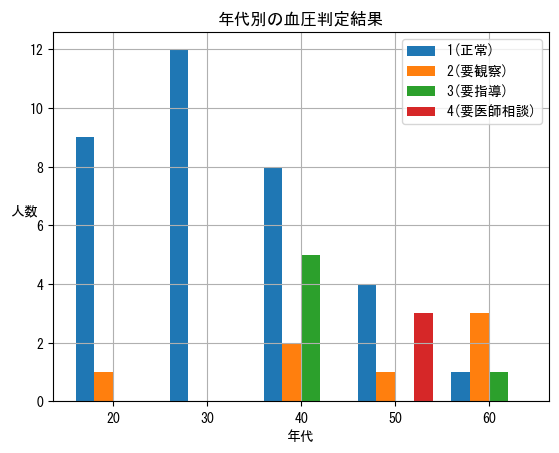
\includegraphics[scale=0.7]{images/allgender/age_bldPrs_result.png}
    \end{figure}

        以下のラフから分かるように、20代から30代にかけては基本的に血圧に問題の無い人しかいない。しかし、40代以上の年代になると、要観察、要指導、要医師相談のひとの割合が増え、正常な人の割合が減少する傾向にあるのが分かる。
        特に、50代のデータで、要医師相談の人の割合が正常の人の割合と近いくらいにまで増えている。加えて、60代では要観察の人の割合が正常な人の割合を上回っているのが分かる。\par 
        このことから、年齢が上がるにつれて、血圧に問題があると判定される人の割合が増えていることが分かる。よって、加齢による老化が原因で、血圧に異常が発生すると考えられる。
            \subsubsection{年代別の心電図判定}
        \begin{figure}[H]
            \centering
            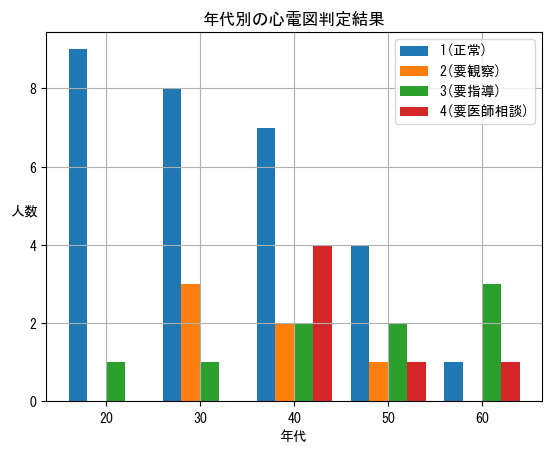
\includegraphics[scale=0.7]{images/allgender/age_heart_result.png}
        \end{figure}
        心電図判定のグラフも、血圧判定のグラフと同様に正常な人の割合は、年齢を上げるにつれて減少し、反対に要観察や要指導、要医師相談の人の割合が増加していることが分かる。\par
        ここで、40代のグラフに注目してほしい。血圧判定のグラフでは、40代の場合要医師相談の人の割合は無かったが、心電図判定のグラフでは、要医師相談の人の割合が急増しており、正常な人の割合
        の半分程度に昇っているのが分かる。\par 
        このことから、血圧異常の前に、心電図に医療機関の受診を勧めるレベルの異常が発生すると考えられる。加えて、40代より上の年代では、心電図が正常な人の割合が激減している。
        このことから、40代後半より心臓になんらかの異常をきたし、その結果血圧にも徐々に異常をきたすようになってしまうと考えられる。これを裏付ける論文に以下の記載があるので引用する。
        \begin{quote}
            以後40歳ごろまではあまり年齢との関係を認めない(とくに男子)が,45歳を過ぎるころから
            は加齢とともに直線的に漸次減少の一途をたどり,男女の別なく50歳前後では約半数になんらかの異常所見がみられるようである
            \begin{figure}[H]
                \centering
                    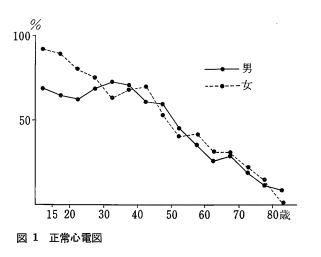
\includegraphics[scale=0.9]{images/allgender/cap.png}
                    \caption{正常な心電図の年代別割合の推移}
            \end{figure}
            ※引用元: 「加齢と心電図」(著)久保 田昌良, 武信満喜夫,島本多喜雄 \url{https://www.jstage.jst.go.jp/article/shinzo1969/2/3/2_278/_pdf} 。
        \end{quote}
        よって、上の論文と本データのグラフから、年齢を重ねるにつれて心電図の正常な人の割合は減少し、特に40歳後半から心臓になんらかの異常が発生する人の割合が増えるため、その後50代、60代で血圧の異常に結びついていると考えられる。
        
\section{各数値データの相関比}
    全性別において、各数値(量的)データと質的データの相関比を算出したのでその結果と考察を以下に示す。
    \subsection{体重と血圧判定の関係}
    \begin{table}[H]
        \centering
        \begin{tabular}{r|c}
            & 血圧判定との相関比 \\ \hline
        年齢   & 0.54 \\
        身長   & 0.19 \\
        体重   & 0.53 \\
        最大血圧 & 0.85 \\
        最小血圧 & 0.55
        \end{tabular}
        \caption{全性別における各数値データと血圧判定の相関比}
    \end{table}
    この結果から、血圧以外の各数値データのうち、血圧判定と関連性のある属性は「年齢」と「体重」であることが分かる。
    年齢と血圧判定の関係性に関しては、先に示した年齢と血圧判定の集計のグラフから読み取ることが出来る。\par
        では、体重と血圧判定に関してはどうだろうか。相関比の数値上では年齢と同程度の関連性があると読み取れるが、実際にグラフに書き起こすと以下のような結果を得た。
        \begin{figure}[H]
            \centering
            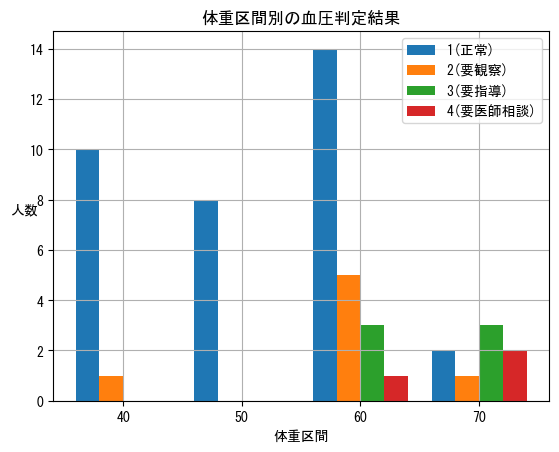
\includegraphics[scale=0.7]{images/allgender/weight_bldPrs_result.png}
        \end{figure}
        一見では、年齢と同程度の関連性を見出すことはできない。しかし、体重60kgを超えた人から、徐々にではあるが要観察、要指導、要医師相談の人の割合が増加しているように見える。
        加えて、70kg代のデータにおいては、正常と判定された人の割合が激減している。\par 
        このことから、体重と血圧測定の関係に関して、体重60kgまでならば血圧に異常はなく、体重が70kg以上になると血圧に問題を生じる確率が高くなると考えることが出来る。
        これを裏付ける資料として以下の文を引用する。
        \begin{quote}
            内蔵脂肪型肥満では、脂肪細胞が分泌する物質や交感神経の活動亢進(活発になること)による血管の収縮、過食や塩分の取りすぎによる体液量の増加、およびインスリンの効きが悪くなるために過剰に分泌されたインスリンにより、腎臓での塩分調整障害が起こり体液量が増加するなど、血圧を上げる働きが多くなり結果として血圧が上昇します。
            \begin{figure}[H]
                \centering
                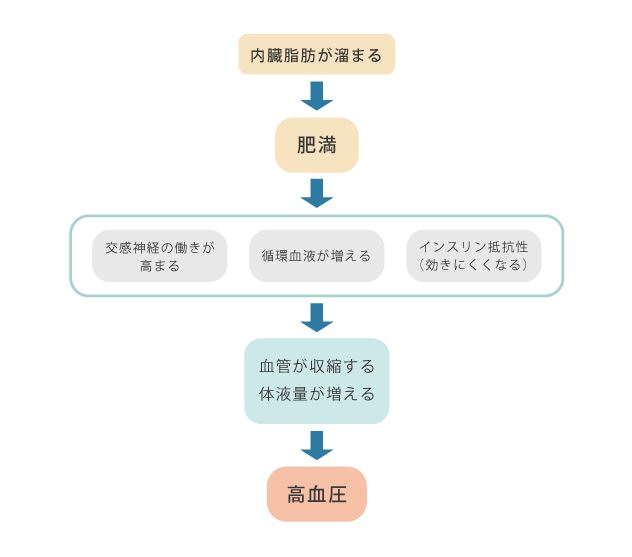
\includegraphics[scale=0.5]{images/allgender/cap2.JPG}
                \caption{肥満から高血圧へ至るまでのフロー図}
            \end{figure}
            ※引用元:\url{https://fukushima-mimamori.jp/physical-examination/column/06.html}
        \end{quote}
        つまり、体重が70kg以上のいわゆる「肥満」に該当する人の場合、交感神経の活動による血管の収縮やインスリンの過剰分泌により、血圧に異常をきたすという事だ。\par 
        よって、グラフと引用文から、体重と血圧判定の相関比が年齢と同程度の関連性になった理由として、体重の増加による、体内環境の変化(交感神経の活動、インスリンの過剰分泌)により、高血圧となる人が増えたため、と考えることが出来る。
    \subsection{体重と心電図判定の関係}
    次に、各数値データと心電図判定の相関比を算出した結果を示す。
    \begin{table}[H]
        \centering
        \begin{tabular}{r|c}
            & 心電図判定との相関比 \\ \hline
        年齢   & 0.44       \\
        身長   & 0.22       \\
        体重   & 0.56       \\
        最大血圧 & 0.78       \\
        最小血圧 & 0.66      
        \end{tabular}
        \caption{全性別における各数値データと心電図判定の相関比}
    \end{table}
    この結果から、各数値データのうち、心電図判定と関連性のある属性は「年齢」と「体重」に加え「最大・最小血圧」であることが分かる。
    年齢と心電図判定の関係性に関しては、先に示した年齢と心電図判定の集計のグラフから読み取ることが出来る。\par
    では、体重、最大最小血圧値に関してはどうだろうか。実際にグラフに書き起こすと以下のような結果を得た。\par
    \paragraph{体重と心電図判定}
    \begin{figure}[H]
        \centering
        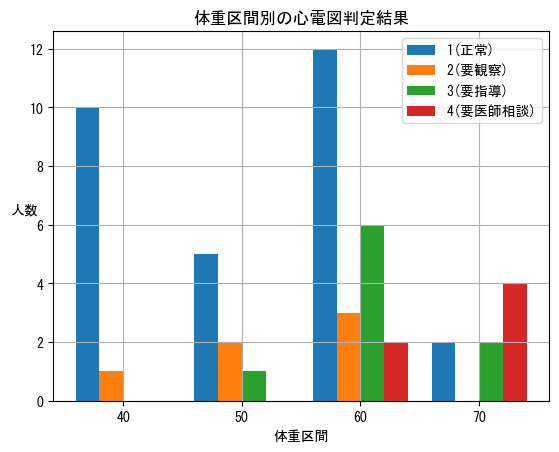
\includegraphics[scale=0.7]{images/allgender/weight_heart_result.png}
    \end{figure}
    

\end{document}